\definecolor{cOne}{HTML}{4C78A8}
\definecolor{cTwo}{HTML}{F58518}
\definecolor{cThree}{HTML}{54A24B}
\definecolor{cFour}{HTML}{8E6BBE}
\definecolor{tfgrey}{HTML}{9CA3AF}
\definecolor{tfsoft}{HTML}{F3F4F6}

\providecommand{\melnode}[4]{%
  \fill[#3!30] (#1,#2) circle (0.42);
  \draw[#3!90!black, line width=0.7pt] (#1,#2) circle (0.42);
  \node[text=#3!80!black, font=\scriptsize] at (#1,#2) {$#4$};
}

\resizebox{\textwidth}{!}{%
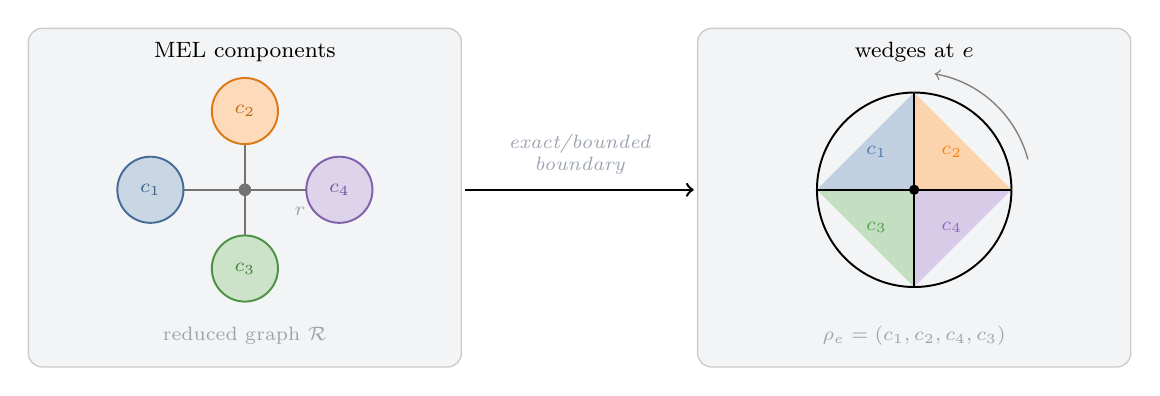
\begin{tikzpicture}[font=\rmfamily\footnotesize]

  % --------------------------------------------------------------------------
  % Panels
  % --------------------------------------------------------------------------
  \fill[tfsoft, rounded corners=5pt] (-7.00,-1.70) rectangle (-1.50,2.60);
  \fill[tfsoft, rounded corners=5pt] ( 1.50,-1.70) rectangle ( 7.00,2.60);
  \draw[black!20, line width=0.5pt, rounded corners=5pt] (-7.00,-1.70) rectangle (-1.50,2.60);
  \draw[black!20, line width=0.5pt, rounded corners=5pt] ( 1.50,-1.70) rectangle ( 7.00,2.60);

  \node[font=\footnotesize] at (-4.25,2.30)
    {MEL components};

  \node[font=\footnotesize] at (4.25,2.30)
    {wedges at $e$};

  % --------------------------------------------------------------------------
  % LEFT: MEL components + a relation r between them.
  % --------------------------------------------------------------------------
  \coordinate (rcenter) at (-4.25,0.55);
  \draw[black!55, line width=0.9pt] (-5.45,0.55) -- (rcenter);
  \draw[black!55, line width=0.9pt] (rcenter) -- (-4.25,1.55);
  \draw[black!55, line width=0.9pt] (rcenter) -- (-3.05,0.55);
  \draw[black!55, line width=0.9pt] (rcenter) -- (-4.25,-0.45);
  \fill[black!55] (rcenter) circle (0.08);
  \node[font=\scriptsize, text=tfgrey] at (-3.55,0.28) {$r$};

  \melnode{-5.45}{ 0.55}{cOne}{c_1}
  \melnode{-4.25}{ 1.55}{cTwo}{c_2}
  \melnode{-3.05}{ 0.55}{cFour}{c_4}
  \melnode{-4.25}{-0.45}{cThree}{c_3}

  \node[font=\scriptsize, align=center, text=tfgrey] at (-4.25,-1.30)
    {reduced graph $\mathcal{R}$};


  % --------------------------------------------------------------------------
  % RIGHT: wedges at the non-manifold edge -- one cross-section, four
  % face-sectors coloured by their owning MEL component.
  % --------------------------------------------------------------------------
  \begin{scope}[shift={(4.25,0.55)}, scale=1.30]
    \draw[black, line width=0.7pt] (0,0) circle (0.95);
    \fill[cTwo!35]   (0,0) -- (90:0.95) -- (0:0.95) -- cycle;
    \fill[cFour!35]  (0,0) -- (0:0.95) -- (-90:0.95) -- cycle;
    \fill[cThree!35] (0,0) -- (-90:0.95) -- (180:0.95) -- cycle;
    \fill[cOne!35]   (0,0) -- (180:0.95) -- (90:0.95) -- cycle;

    \node[text=cTwo,   font=\scriptsize] at (45:0.52)   {$c_2$};
    \node[text=cFour,  font=\scriptsize] at (-45:0.52)  {$c_4$};
    \node[text=cThree, font=\scriptsize] at (-135:0.52) {$c_3$};
    \node[text=cOne,   font=\scriptsize] at (135:0.52)  {$c_1$};

    \draw[black, line width=0.6pt] (0,0) -- (90:0.95);
    \draw[black, line width=0.6pt] (0,0) -- (0:0.95);
    \draw[black, line width=0.6pt] (0,0) -- (-90:0.95);
    \draw[black, line width=0.6pt] (0,0) -- (180:0.95);
    \fill[black] (0,0) circle (0.05);

    % Cyclic order hint (small arc arrow around the rim).
    \draw[->, black!50, line width=0.5pt]
      (15:1.15) arc[start angle=15, end angle=80, radius=1.15];
  \end{scope}

  \node[font=\scriptsize, align=center, text=tfgrey] at (4.25,-1.30)
    {$\rho_e = (c_1, c_2, c_4, c_3)$};

  % --------------------------------------------------------------------------
  % Bridge between the two boxes.
  % --------------------------------------------------------------------------
  \draw[->, line width=0.9pt, black]
    (-1.45,0.55) -- (1.45,0.55);

  \node[font=\scriptsize\itshape, align=center, text=tfgrey] at (0,1.00)
    {exact/bounded\\boundary};

\end{tikzpicture}%
}
